\section*{Problem 5}

State is $z=[x,\theta,\dot x,\dot\theta]^T$, and I use $D=I(M+m)+Mml^2=(m+M)(I+ml^2)-m^2l^2$.

\subsection*{1. Small-angle linearization}

With $\cos\theta\approx1$, $\sin\theta\approx\theta$ and $\dot\theta^2\sin\theta\approx0$ the equations become
\[
(m+M)\ddot x+ml\ddot\theta=F,\qquad (I+ml^2)\ddot\theta+ml\ddot x=mgl\,\theta .
\]
Solving the two for the accelerations:
\[
\ddot x=\frac{(I+ml^2)F-m^2gl^2\theta}{D},\qquad
\ddot\theta=\frac{mgl(M+m)\theta-mlF}{D}.
\]
\[
A=\bmat{0&0&1&0\\0&0&0&1\\0&-\frac{m^2gl^2}{D}&0&0\\0&\frac{mgl(M+m)}{D}&0&0},\qquad
B=\bmat{0\\0\\\frac{I+ml^2}{D}\\-\frac{ml}{D}}
\]

\subsection*{2. Nonlinear form and Taylor expansion}

Solving the exact equations for $\ddot x$ and $\ddot\theta$, with $\Delta(\theta)=D+m^2l^2\sin^2\theta$:
\begin{align*}
\ddot x&=\frac{(I+ml^2)F+ml(I+ml^2)\dot\theta^2\sin\theta-m^2gl^2\sin\theta\cos\theta}{\Delta(\theta)},\\
\ddot\theta&=\frac{ml\,[\,-F\cos\theta+(M+m)g\sin\theta-ml\dot\theta^2\sin\theta\cos\theta\,]}{\Delta(\theta)},
\end{align*}
and $\dot z=[\dot x,\dot\theta,\ddot x,\ddot\theta]^T$. At $z=0$, $F=0$ both numerators are zero, so the derivative of $\Delta$ does not matter, and $\partial\Delta/\partial\theta=0$ there anyway. The terms with $\dot\theta^2$ vanish as well. What is left is
\[
\frac{\partial\ddot x}{\partial\theta}=-\frac{m^2gl^2}{D},\quad
\frac{\partial\ddot\theta}{\partial\theta}=\frac{mgl(M+m)}{D},\quad
\frac{\partial\ddot x}{\partial F}=\frac{I+ml^2}{D},\quad
\frac{\partial\ddot\theta}{\partial F}=-\frac{ml}{D},
\]
which is the same $A$ and $B$ as in part 1. The code also checks this symbolically.

\subsection*{3. State feedback}

With $m=0.16$, $M=0.48$, $l=0.5$, $g=9.8$, $I=\tfrac1{12}ml^2$:
\[
A=\bmat{0&0&1&0\\0&0&0&1\\0&-2.94&0&0\\0&23.52&0&0},\qquad
B=\bmat{0\\0\\2.03125\\-3.75}.
\]
The open-loop eigenvalues are $0,0,\pm4.85$, so it is unstable. The controllability matrix has full rank (4), so poles can be placed anywhere. I picked $\{-2,-3,-4,-5\}$, i.e.\ $s^4+14s^3+71s^2+154s+120$, and got
\[
K=\bmat{-3.265&-26.974&-4.190&-6.003},\qquad F=-Kz .
\]
I also simulated the full nonlinear model with this controller from $\theta_0=0.1$ and $0.3$\,rad, and both go back to zero (Fig.~\ref{fig:p5}).

\textbf{Symbolic gain (bonus).} Write $a=-\tfrac{m^2gl^2}{D}$, $b=\tfrac{mgl(M+m)}{D}$, $c=\tfrac{I+ml^2}{D}$, $d=-\tfrac{ml}{D}$. Expanding $\det(sI-A+BK)$ gives
\[
s^4+(ck_3+dk_4)s^3+(-b+ck_1+dk_2)s^2+(ad-bc)k_3\,s+(ad-bc)k_1 ,
\]
and $ad-bc=-glm/D$. Matching to $s^4+p_3s^3+p_2s^2+p_1s+p_0$:
\[
k_1=-\frac{D\,p_0}{glm},\quad
k_3=-\frac{D\,p_1}{glm},\quad
k_2=\frac{p_2+b-c\,k_1}{d},\quad
k_4=\frac{p_3-c\,k_3}{d}.
\]
Plugging in the numbers gives the same $K$ as \texttt{place}.

\begin{lstlisting}
A0 = simplify(subs(jacobian(f, z), vars, [0 0 0 0 0]));   % Taylor
B0 = simplify(subs(diff(f, F),     vars, [0 0 0 0 0]));
K  = place(An, Bn, [-2 -3 -4 -5]);
cp = expand(det(s*eye(4) - (A_s - B_s*[k1 k2 k3 k4])));
Ks = solve(coeffs(cp - cdes, s), [k1 k2 k3 k4]);          % symbolic gains
\end{lstlisting}

\begin{figure}[h]
\centering
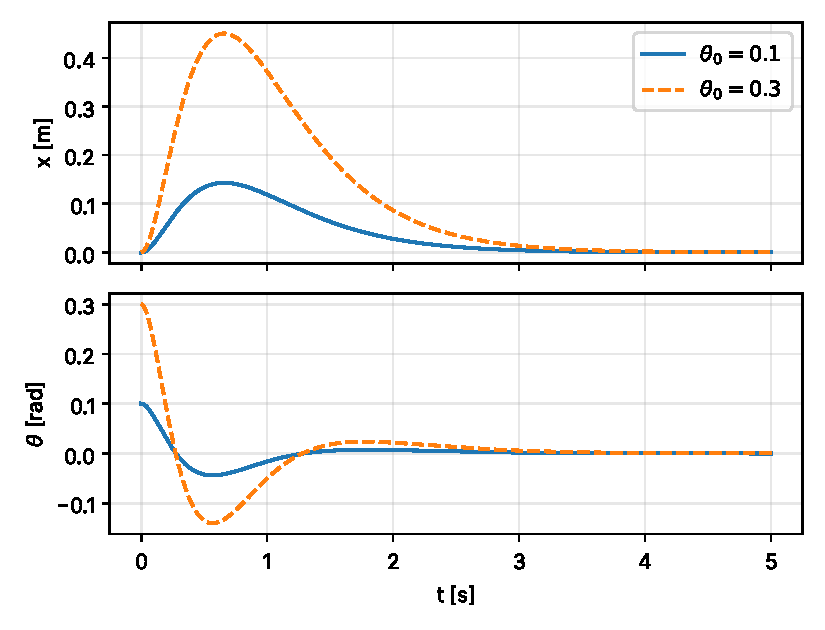
\includegraphics[width=0.6\linewidth]{figures/p5.pdf}
\caption{Nonlinear cart-pendulum with $F=-Kz$.}
\label{fig:p5}
\end{figure}

\subsection*{4. (Bonus) Equations of motion}

Take the pendulum center of mass at $(x+l\sin\theta,\;l\cos\theta)$. Then
\[
T=\tfrac12(M+m)\dot x^2+ml\dot x\dot\theta\cos\theta+\tfrac12(I+ml^2)\dot\theta^2,\qquad V=mgl\cos\theta,
\]
and the generalized forces are $Q_x=F$, $Q_\theta=0$. Lagrange's equation for $x$ gives $(M+m)\ddot x+ml\ddot\theta\cos\theta-ml\dot\theta^2\sin\theta=F$. For $\theta$ the $ml\dot x\dot\theta\sin\theta$ terms cancel and you get $(I+ml^2)\ddot\theta+ml\ddot x\cos\theta-mgl\sin\theta=0$. Both match the given equations.

\subsection*{5. (Bonus) Linearization at $\theta=\pi$}

Let $\varphi=\theta-\pi$, so $\sin\theta\approx-\varphi$ and $\cos\theta\approx-1$:
\[
(m+M)\ddot x-ml\ddot\varphi=F,\qquad (I+ml^2)\ddot\varphi-ml\ddot x+mgl\,\varphi=0 .
\]
Solving gives
\[
\ddot x=\frac{(I+ml^2)F-m^2gl^2\varphi}{D},\qquad
\ddot\varphi=\frac{mlF-mgl(M+m)\varphi}{D}.
\]
So $A$ is the same as before except the $(4,2)$ entry flips sign, and the last entry of $B$ is $+ml/D$. The Taylor expansion gives the same thing. Now the lower block is oscillatory, $\lambda=\pm j4.85$, which makes sense for a pendulum hanging down.
